\chapter{Analiza możliwych rozwiązań}
\label{cha:możliwe_układy}
 W~poprzednim rozdziale autor pokazał możliwe struktury układu tłumienia hałasu -- pasywny lub aktywny. W~tym rozdziale, autor wybiera konstrukcję hybrydową (pasywno-aktywną) feedforward-feedback oraz przedstawi możliwe do zastosowania platformy sprzętowe. Na podstawie analizy słabych i~mocnych stron wymienionych podejść, dokonany zostanie dalszy wybór.

 Zasada konstrukcyjna systemu aktywnego tłumienia hałasu w~żadnym kroku nie specyfikuje układu elektronicznego, na którym można zaimplementować algorytm tłumienia. Oznacza to zatem, że jeżeli konstruktor zastosuje się do praw fizyki i~wymagań projektu, to powinien być w~stanie zaimplementować cały system na dowolnym układzie -- analogowym lub cyfrowym. W~następnych sekcjach autor postara się odpowiedzieć na pytanie -- który z~nich najlepiej wybrać, a~jeśli cyfrowy, to jaka platforma sprzętowa jest najlepsza? 
\section{Układ analogowy}
\label{sec:analog}
Układ analogowy jest najtańszy i~najszybszy -- bazuje na wzmacniaczach operacyjnych odwracających i~odpowiednim wysterowaniu fazy sygnału. Daje możliwość osiągnięcia wysokich zakresów częstotliwościowych oraz charakteryzuje się bardzo niskim poborem prądu -- co sprzyja dobrej praktyce projektowania układów tanich w~zasilaniu, co ma szczególne znaczenie przy zasilaniu bateryjnym. Pojawiają się jednak problemy przy implementowaniu pętli automatyki adaptacyjnego filtru -- złożoność układu znacznie wzrasta, trudno jest też poprawić taki system, jeśli gdzieś popełniono błąd. W~zasadzie nie da się takiego rozwiązania zaprojektować inkrementacyjnie -- należy opracować od razu cały, kompletny system, gdyż zmiany w~trakcie konstruowania wymagają zbudowania całości od nowa. Choć rozwiązanie jest mniej kosztowne i szybsze od innych, jest też zadziwiająco nieelastyczne, a~przy wzrastającej złożoności filtra komplikuje się jego konstrukcja.
\section{Układ cyfrowy}
\label{sec:digital}
Zastosowanie cyfrowego układu może być droższe i~wydaje się nieco trudniejsze, jednak zwiększa możliwości konstrukcyjne. Do wyboru jest wiele platform, bardzo często integrujących w~sobie sporo funkcjonalności, które w~podejściu analogowym należałoby samodzielnie stworzyć (zakładając oczywiście, że technika analogowa na to pozwoli).  Pomimo początkowego zwiększenia złożoności systemu, okazuje się, że w~dłuższej perspektywie czasowej ułatwione jest jego prototypowanie i~programowanie, ponieważ istnieje mnogość narzędzi inżynierskich pomagających w~procesie pracy z~układami cyfrowymi. Można nawet powiedzieć, że ucyfrowienie platformy realizującej tłumienie hałasu daje szansę na zaimplementowanie wymiennych algorytmów, filtrów i~dodanie kilku funkcjonalności, czyli uczynienie systemu modułowym i~przystosowanym do różnych zastosowań. Taka jest zresztą zasada działania kart dźwiękowych, które posiadają zaawansowane silniki efektów, swobodnie dodawane, usuwane i~modyfikowane. W~odróżnieniu od ścieżki analogowej, układ taki jest też zdecydowanie mniej podatny na szumy, przesłuch i~przydźwięk sieciowy ze względu na charakter przesyłanego sygnału. Następne sekcje przybliżą przykłady platform, które pozwoliłyby na realizację układu aktywnego tłumienia hałasu.
\subsection{Mikrokontroler}
\label{uC}
Odpowiednio złożonym, a~jednocześnie niezbyt skomplikowanym układem jest mikrokontroler. Jedną z~najbardziej popularnych obecnie grup mikrokontrolerów jest rodzina urządzeń STM32, bazujących na mikroprocesorach ARM~Cortex-M4. Warto nadmienić, że firma STMicroelectronics posiada w~asortymencie zarówno same mikrokontrolery, jak i~płytki prototypowe z~zamontowanymi gotowymi peryferiami. Ta platforma udostępnia dwa możliwe sposoby programowania:
\begin{itemize}
	\item bare-metal programming -- czyli programowanie czystego sprzętu na zasadzie proceduralnej bez zainstalowanego systemu operacyjnego,
	\item RTOS\footnote{System operacyjny czasu rzeczywistego (ang. Real-Time Operating System)} -- czyli instalacja i~obsługa odwołań systemu posiadającego jądro czasu rzeczywistego i~wspierającego tego typu zastosowania.
\end{itemize}
Ponieważ projekt nie wymaga posiadania systemu operacyjnego, rozważa się tutaj tylko podejście bare-metal programming. Twórcy opisywanej platformy regularnie dostarczają nowe płytki prototypowe, narzędzia, programy oraz biblioteki programistyczne, które tworzą efektywny i~spójny ekosystem ułatwiający pracę.
\subsection{Mikrokomputer jednopłytkowy}
\label{mikrokomp}
Taka platforma jest o~jeden krok bardziej zaawansowana od mikrokontrolera -- zazwyczaj zawiera wiele układów peryferyjnych oraz daje możliwość zainstalowania pełnego systemu operacyjnego Linux, Windows i~tym podobnych. Mikrokomputery zazwyczaj posiadają bardziej zaawansowane komponenty, więcej pamięci i~szybsze procesory. Ponieważ mikrokomputery mają zainstalowany system operacyjny, można dowolnie dobrać środowisko programistyczne, implementować dodatkowe funkcjonalności oraz wykorzystać systemowe wsparcie dla wielowątkowości. Można by na przykład użyć jednego wątku do algorytmu aktywnego tłumienia hałasu, zaś na drugim zbierać statystyki i~przesyłać je chociażby do pliku lub serwisu sieciowego, by później przetworzyć te dane.

Niestety okazuje się, że narzut czasowy powstały w~wyniku wprowadzenia do projektu systemu operacyjnego jest zbyt duży -- należy w~pierwszej kolejności zwrócić uwagę na fakt, że zwykły system (nie czasu rzeczywistego) ma niewywłaszczalne jądro. Oznacza to, że proces jądra, który raz zacznie być przetwarzany, musi być dokończony, i~nie da się go przerwać. Z~kolei system, który ma wywłaszczalne jądro, wspiera rozróżnianie priorytetów procesów -- co sprawia, że w~momencie przyjścia przerwania od ,,ważniejszego'' procesu, ten o~niższym priorytecie oddaje zasób. Pozwala to, poprzez modyfikację priorytetów w~jądrze systemu, ustawić największe prawa dla sterownika dźwięku.
Autor, pragnąc poprzeć powyższy wywód eksperymentem, przeprowadził prosty test opóźnienia na mikrokomputerze Raspberry~Pi~3B+. Na sprzęcie zainstalowano system operacyjny Raspbian~Lite, bazujący na systemie operacyjnym Linux (dystrybucja Debian), który, choć nie jest systemem czasu rzeczywistego, to dość mocno obniża zużycie zasobów poprzez wyłączenie w~konfiguracji większości daemonów\footnote{daemon -- proces działający w tle, zazwyczaj jest to sterownik sprzętu, na przykład sterownik Bluetooth} i~pozostawienie tylko najpotrzebniejszych (do działania projektu -- a~więc sterowników dźwięku). Do przeprowadzenia testu opóźnienia wykorzystano API sterownika ALSA\footnote{Zaawansowana Architektura Dźwięku dla Linux (ang. Advanced Linux Sound Architecture)}. Wśród przykładowych programów (napisanych w~języku C) można znaleźć plik nazwany \textit{latency.c}\footnote{https://www.alsa-project.org/wiki/Test\_latency.c -- stan z~dnia 25.11.2019 godzina 15:00}, który dla kilku podstawowych częstotliwości dźwięku wylicza opóźnienie przesłania sygnału z~wejścia (mikrofonu) bezpośrednio na wyjście (głośnik). Okazało się, że opóźnienia wyniosły około 3-4 ms dla częstotliwości \SI{500}{\Hz}, co całkowicie wyklucza zastosowanie tej platformy. Jedynym sposobem uniknięcia takich narzutów czasowych jest zastosowanie niskopoziomowego systemu czasu rzeczywistego, jednak to zredukowałoby charakter platformy sprzętowej do poziomu mikrokontrolera.
\subsection{Karta dźwiękowa komputera PC}
\label{soundcard}
Podstawowa karta dźwiękowa zawiera cztery główne elementy:
\begin{enumerate}
	\item Wejścia i~wyjścia do komunikacji z~mikrofonami lub głośnikami (lub podobnymi urządzeniami).
	\item Wielokanałowy przetwornik analogowo-cyfrowy (dokonuje konwersji sygnałów wejściowych).
	\item Wielokanałowy przetwornik cyfrowo-analogowy (dokonuje konwersji sygnałów wyjściowych).
	\item Interfejs PCI\footnote{Magistrala komunikacyjna (ang. Peripheral Component Interconnect) przyłączająca karty rozszerzające do płyty głównej komputera} lub inny, zazwyczaj używany do komunikacji z~płytą główną komputera, w~którym zainstalowana jest karta.
\end{enumerate}
Większość nowoczesnych kart dźwiękowych zawiera jednak znacznie więcej niż wymienione komponenty, aby zapewnić wsparcie dla zaawansowanych funkcjonalności, takich jak dźwięk stereofoniczny 3D, wsparcie dla MIDI\footnote{Cyfrowy interfejs instrumentów muzycznych (ang. Musical Instrument Digital Interface)}, dodatkowe efekty dźwiękowe i~wiele innych. Wśród komponentów można znaleźć na przykład procesory DSP\footnote{Procesor sygnałowy (ang. Digital Signal Processor)} lub nawet zaawansowane silniki dźwiękowe, dedykowane do~dokonywania przetworzeń dźwięku w~dziedzinie czasu lub częstotliwości (jak na przykład dodanie echa, opóźnienia czasowego, miksowanie efektów lub filtracja). Takie silniki stosowane są na przykład w~kartach dźwiękowych firmy Creative, by odciążyć główny procesor i~przyspieszyć konwersje.\\
Z~uwagi na przeznaczenie kart dźwiękowych oraz różnorodność oferowanych przez nie funkcji, wydawać by się mogło, że są one idealnymi kandydatami na platformę sprzętową do układu aktywnego tłumienia hałasu. Tak jednak nie jest ze względu na niedostępność tej platformy -- twórcy kart dźwiękowych raczej nie udostępniają żadnych możliwości ingerowania w~oprogramowanie, zostawiając jedynie możliwość tworzenia sterowników obsługujących efekt działania kart poprzez oficjalne API\footnote{Interfejs programowania aplikacji (ang. Application Programming Interface)}. Ponadto typowa karta dźwiękowa posiada znaczne gabaryty, wysoką cenę, duże zapotrzebowanie na energię elektryczną i nie jest urządzeniem samodzielnym. To dyskwalifikuje ją w rozważanym zastosowaniu.
\subsection{Układ FPGA}
\label{FPGA}
Bardzo zaawansowana technologia układów FPGA\footnote{Bezpośrednio Programowalna Macierz Bramek (ang. Field Programmable Gate Array)} może być odpowiedzią na problemy z~brakiem wielowątkowości poprzednich rozwiązań. Ta platforma wspiera wielozadaniowość, obliczenia równoległe i~potokowe przetwarzanie danych na poziomie swojej architektury -- jak wskazuje nazwa, opiera się ona na rozległej macierzy programowalnych bramek logicznych. Twórcy tych platform dostarczają własne środowiska programistyczne, gdzie konstruktorzy i~programiści mogą często w~graficzny sposób konfigurować i~programować układy, co ułatwia nieco pracę z~tym zaawansowanym sprzętem. Wiodącym producentem na rynku jest obecnie firma Xilinx, która udostępnia narzędzia programistyczne takie jak Vivado. Niestety, wraz z~możliwościami sprzętu, w~parze idzie jego koszt. Ponieważ dodatkowo konkurencyjność rynku jest niska, producenci tego sprzętu mają swobodę dyktowania wysokich cen -- co zdecydowanie deklasuje to rozwiązanie w~kontekście tego projektu. Pomijając kwestię znacznych kosztów takiej platformy, daje ona zwyczajnie zbyt dużo możliwości, by można ją było wykorzystać jedynie do projektu opartego na przetwarzaniu potokowym. Byłby to przypadek niedopasowania platformy do potrzeb projektu.
\section{Wybór rozwiązania}
\label{sec:wybór}
Autor, biorąc pod uwagę wymienione zalety i~wady, koszty oraz przeprowadzone testy, zdecydował się na rozwiązanie postawionego problemu inżynierskiego przy użyciu platformy mikrokontrolera bez zainstalowanego systemu operacyjnego -- metodą bare-metal programming. Wybrał do tego celu płytkę prototypową NUCLEO-F446RE z~mikrokontrolerem STM32F446RE, zawierającą wszystkie niezbędne do realizacji projektu komponenty. Autor motywuje swoją decyzję faktem, iż ta platforma daje dużą swobodę w~projektowaniu rozwiązań i~dostarcza kompletny, darmowy ekosystem programistyczny, pozwalający na szybkie i~łatwe konfigurowanie oraz programowanie tego sprzętu. Dodatkowo, mikrokontroler bez systemu operacyjnego gwarantuje, iż wykonywane będzie tylko to, co konstruktor zaprogramuje. Pozwala to uniknąć narzutów czasowych powstałych od zadań pobocznych i~zostawia programistę z~mniejszą liczbą czynników, które trzeba rozważyć podczas implementowania programu. W~zestawie uruchomieniowym, obok mikrokontrolera przeznaczonego do programowania przez użytkownika, producent umieścił również programator-debugger ST-Link V2-1. Zmniejsza to koszty rozwiązania i~zwiększa wygodę użycia zestawu.
\subsection{Dobór środowiska programistycznego}
\label{sec:IDE}
Jak wspomniano w~poprzedniej sekcji, firma STMicroelectronics dostarcza darmowe, kompletne środowisko programistyczne wspomagające pracę z~jej produktami.\\
Autor postanowił skorzystać z~następujących programów:
\begin{enumerate}
	\item STM32CubeMX (rys. \ref{fig:cubemx})\\
	\begin{figure}[h!]
		\centering
		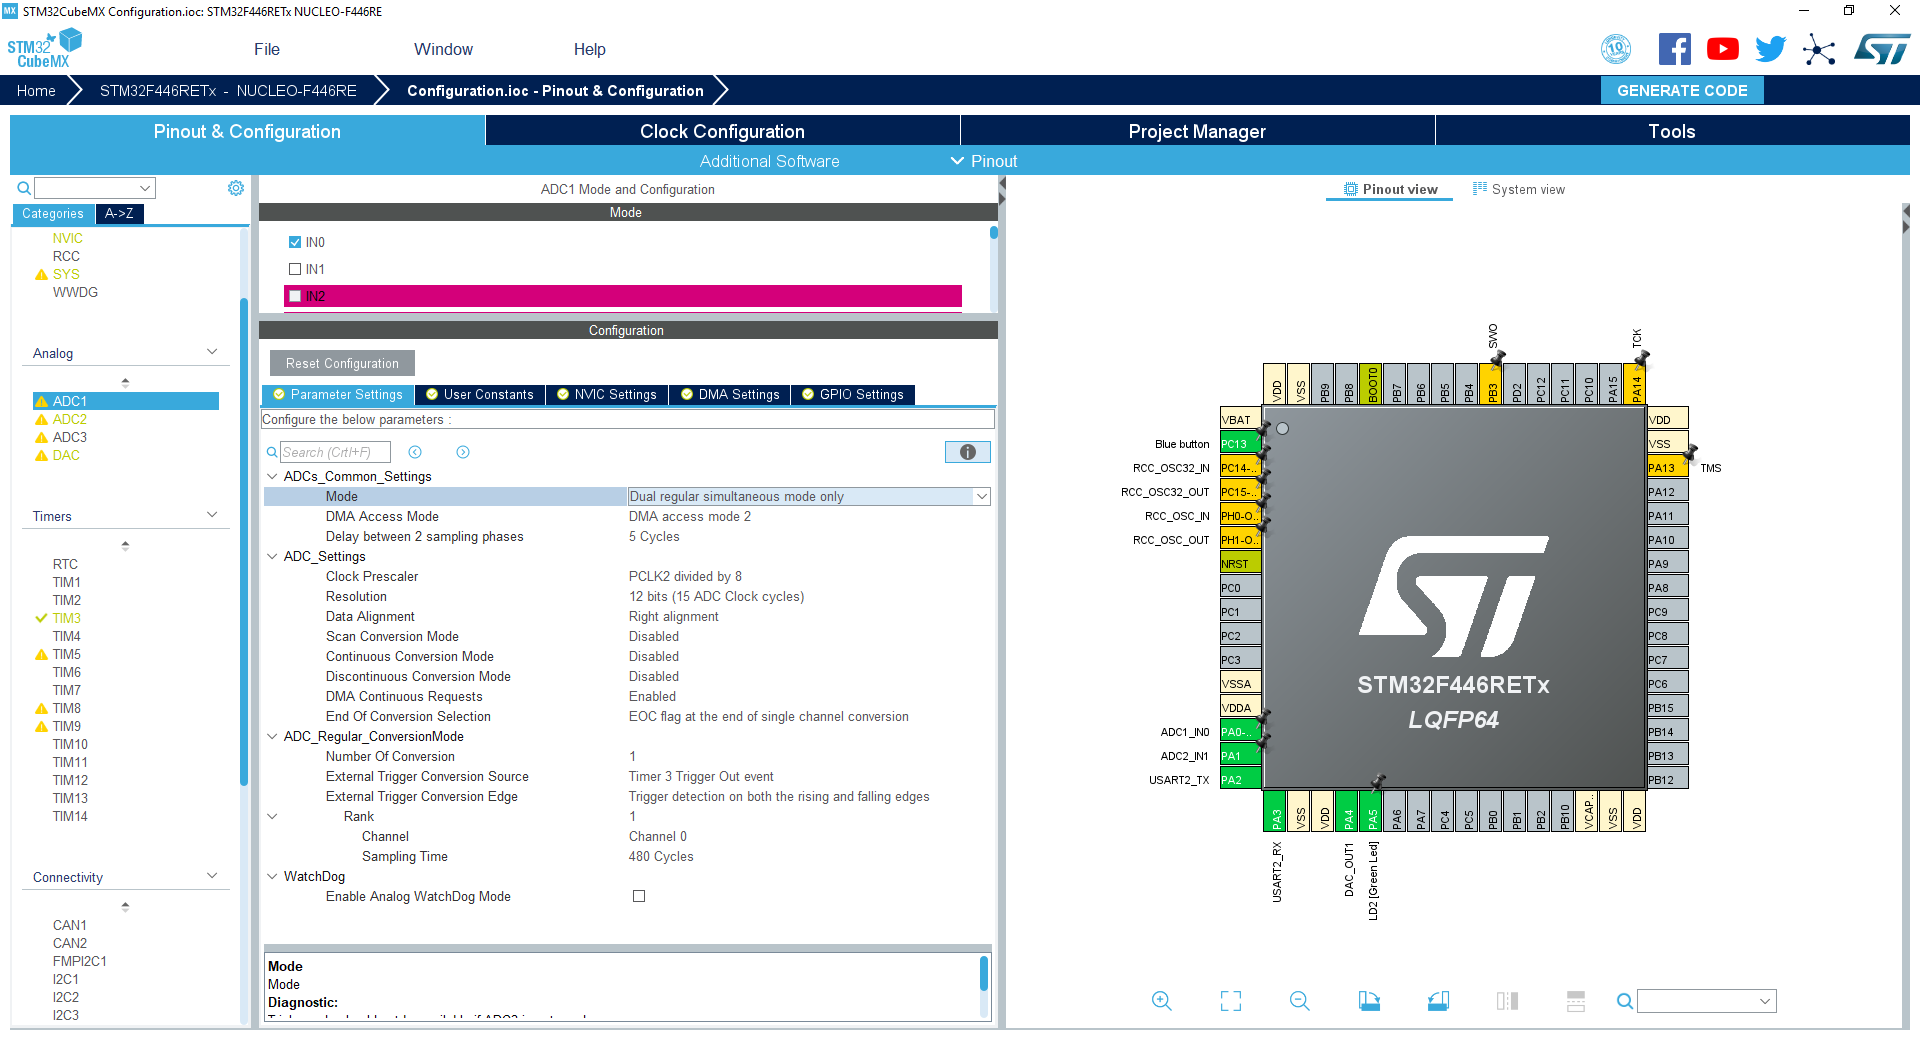
\includegraphics[scale=0.3]{../Assets/stm32CubeMX.png}
		\caption{Okno programu STM32CubeMX z~widokiem na konfigurację przetwornika ADC oraz wyprowadzenia mikrokontrolera.}
		\label{fig:cubemx}
	\end{figure}
	Graficzny konfigurator ułatwiający tworzenie projektu oprogramowania dla mikrokontrolera. Umożliwia wybór płytki prototypowej lub samego mikrokontrolera, uruchamianie/wyłączanie komponentów oraz kompletną konfigurację. Interfejs graficzny aplikacji ułatwia wybór funkcji wyprowadzeń mikrokontrolera oraz skonfigurowanie peryferiów (układów czasowo-licznikowych, przetworników A/C i~C/A, modułów komunikacyjnych itd.).
	\item System Workbench for STM32(rys. \ref{fig:sw4stm})\\
	\begin{figure}[h!]
		\centering
		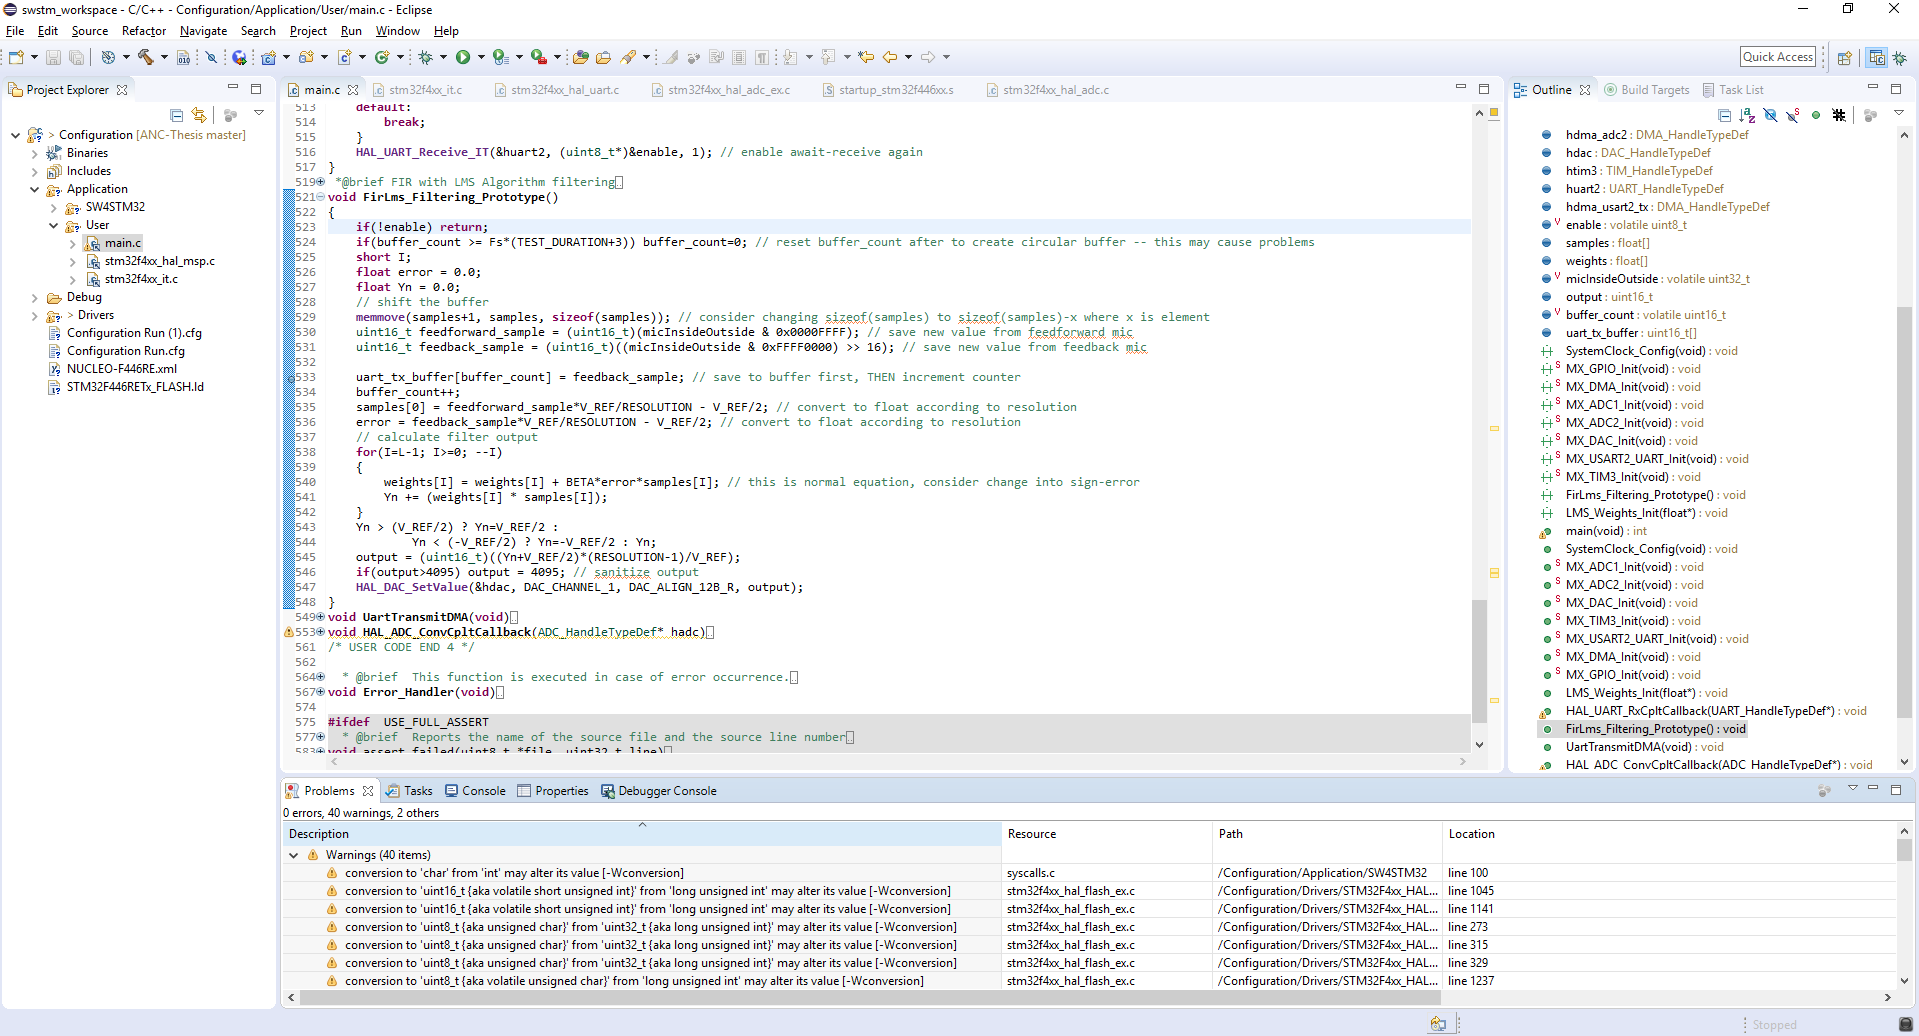
\includegraphics[scale=0.3]{../Assets/sw4stm32.png}
		\caption{Okno programu System Workbench for STM32 z~widokiem na kod programu. Widoczny jest typowy układ środowiska programistycznego Eclipse.}
		\label{fig:sw4stm}
	\end{figure}
	Środowisko programistyczne zrealizowane na bazie Eclipse, stosowane jako samodzielny program lub jako wtyczka do wymienionego środowiska.
	\item STM32 ST-LINK Utility\\
	Program dostarczający interfejsu graficznego oraz tekstowego do programowania i~weryfikacji zawartości pamięci FLASH mikrokontrolera.
	\item STMStudio\\
	Środowisko komunikujące się w~czasie rzeczywistym z~mikrokontrolerem za pomocą obecnego na płytce debuggera/programatora ST-Link. Pozwala na podgląd wartości zmiennych programu w~czasie rzeczywistym oraz wizualizację danych.
\end{enumerate}	